% This is samplepaper.tex, a sample chapter demonstrating the
% LLNCS macro package for Springer Computer Science proceedings;
% Version 2.20 of 2017/10/04
%
\documentclass[runningheads]{llncs}
%
\usepackage{amsmath}
\usepackage{amssymb} % for \therefore
\usepackage{graphicx}
\usepackage{array} % for table cell centering
% Used for displaying a sample figure. If possible, figure files should
% be included in EPS format.
%
% If you use the hyperref package, please uncomment the following line
% to display URLs in blue roman font according to Springer's eBook style:
% \renewcommand\UrlFont{\color{blue}\rmfamily}

\begin{document}
%
\title{An Evaluation of Uninformed and Informed Search Algorithms on the $k$-puzzle Problem}
\subtitle{AY19/20 Semester 2 CS3243 Project 1, Group 37}
%
\titlerunning{Search Algorithms on the $k$-puzzle Problem}
% If the paper title is too long for the running head, you can set
% an abbreviated paper title here
%
\author{Lim Fong Yuan \and
Zhuang Xinjie \and
Otto Alexander Sutianto \and
Mario Lorenzo}
%
\authorrunning{Lim et al.}
% First names are abbreviated in the running head.
% If there are more than two authors, 'et al.' is used.
%
\institute{School of Computing, National University of Singapore% \and
%Springer Heidelberg, Tiergartenstr. 17, 69121 Heidelberg, Germany
%\email{lncs@springer.com}\\
%\url{http://www.springer.com/gp/computer-science/lncs} \and
%ABC Institute, Rupert-Karls-University Heidelberg, Heidelberg, Germany\\
%\email{\{abc,lncs\}@uni-heidelberg.de}
}
%
\maketitle              % typeset the header of the contribution
%
%\begin{abstract}
%The abstract should briefly summarize the contents of the paper in
%150--250 words.

%\keywords{First keyword  \and Second keyword \and Another keyword.}
%\end{abstract}
%
%
%
\section{Problem Specification}
Fix $n \in \bbbz_{\geq 2}$. Let $k = n^2 -1$.
A valid state $v$ is a $n \times n$ array with the entries $v_{(x,y)}$ containing a permutation of the integers $[0,k]$. $V$ is the set of valid states.
Each valid state has a unique coordinate $e = (x_e,y_e)$ such that $v_e = 0$. Call $v_e$ the empty cell of $v$.
The goal state $g$ is where $g_{(x,y)} = (x-1)n+y$ for all $(x,y) \in (\bbbz_{[1,n]})^2$, except for $g_{(n,n)}$ which is $0$.
Let $A = \{\texttt{up}=(-1,0),\texttt{down}=(1,0),\texttt{left}=(0,-1),\texttt{right}=(0,1)\}$ be the set of actions.
The transition function $T: V \times A \to V$ is where $T(v,a) = v'$ with $v'$ being identical to $v$ except with $(v'_{e-a},v'_e) = (v_e,v_{e-a})$.% (Invalid output states are rejected.)

The problem is to determine if $g$ is reachable from a given initial state $s$, and if so, specify a sequence of actions $p \in A^\ast$ (called a solution) that leads from $s$ to $g$.

Throughout this report, the following variable definitions are used:

Let $d$ be the depth of the shallowest goal node $g$.

Let $b$ be the maximum branching factor of the problem space. $b = 3$, see \ref{subsec:branchingfactors}.

%Please try to avoid rasterized images for line-art diagrams and schemas. Whenever possible, use vector graphics instead (see Fig.~\ref{fig1}).
\begin{figure}
	\centering
	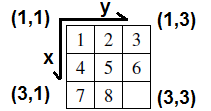
\includegraphics[height=2cm]{coord_system.png}
	\caption{The coordinate system on the goal state, in the case of $n=3$.} \label{fig:coordsystem}
\end{figure}



\section{Technical Analysis}
% Announcement: ``No, you do not need to formally prove the complexity of A* (if used) or any other search algorithm in the textbook, that's not the goal of the project.''
% However, the project specs still say ``Each algorithm implemented should be analysed for correctness and complexity'' (1 mark)

\subsection{Breadth-First Search (BFS) (Uninformed)}

BFS explores all reachable nodes of depth $d'$ before it starts exploring nodes of depth $d'+1$. Hence, there are at most $\sum_{i=0}^d b^i = \frac{b^d-1}{b-1} = \frac{3^d-1}{3-1} \in O(3^d)$ nodes that BFS will explore before it explores $g$.

\subsubsection{Correctness and Optimality}
The algorithm first checks for solvability (see Appendix \ref{subsec:solvability}), terminating if it is not. If a goal node $g$ exists, BFS explores a finite number of nodes before finding the shallowest goal node $g$. Then, it backtracks through its search tree to derive the sequence of actions that leads from $s$ to $g$. All actions that BFS has explored are valid, and the sequence leads from $s$ to $g$, therefore BFS returns a correct sequence.
BFS finds an optimal solution because it explores all nodes of depth $d-1$ before it explores nodes of depth $d$. If there were another solution at depth $d-1$ or closer, BFS would have found it first.

\subsubsection{Efficiency}
Each node is explored in constant time, thus BFS has $O(3^d)$ time complexity. BFS tracks all explored and seen nodes in memory, Which amount to at most $\sum_{i=1}^{d+1} b^i \in O(b^{d+1}) = O(b \cdot b^d) = O(3 \cdot 3^d) = O(3^d)$, thus BFS has $O(3^d)$ space complexity.

\subsection{A* Search (Informed)}

A* explores the node $v$ with the least estimated cost $f(v) = g(v) + h(v)$ to the shallowest goal node $g$, where $g(v)$ is the cost from the initial state $s$ to $v$, and $h(v)$ is an admissible estimate of the cost from $v$ to $g$.

Let $d(v,v')$ be the optimal distance between any two nodes $v$ and $v'$.

Assuming $g$ exists, let $p$ be an optimal path from $s$ to $g$. For any node $v$ in $p$, note that $f(v) = g(v) + h(v) \leq g(v) + h^\ast(v) = d(s,n)+d(n,g) = d(s,g) = d$. Also note that at least one node in $p$ will be in the frontier of A* at any given point, hence there is always at least one node $v$ in the frontier with $f(v) \leq d$. Therefore, A* will explore at most all reachable nodes $v$ such that $f(v) \leq d$ before finding $g$. In particular, it will search at most all nodes $v$ of depth $d' = d(s,v) = g(v) \leq g(v)+h(v) = f(v) \leq d$. Hence, there are at most $\sum_{i=0}^d b^i = \frac{b^d-1}{b-1} = \frac{3^d-1}{3-1} \in O(3^d)$ nodes that A* will explore before it explores $g$.

\subsubsection{Correctness and Optimality}
Same as with BFS above.

\subsubsection{Efficiency}
Same as with BFS above, A* has $O(3^d)$ time and $O(3^d)$ space complexity, in the worst case (i.e. constant heuristic). The time complexity may be improved depending on the heuristic, generally taking on the form $O(b^{d-h(s)})$, or $O((b^\ast)^d)$ (where $b^\ast$ is the effective branching factor of A* using $h$, which has to be empirically measured), see \cite{AIMA-A*Complexity}. At best, under the optimal heuristic $h^\ast$ (where $h^\ast(v)$ returns the actual cost from $v$ to $g$), A* runs in $O(d)$ time.

\subsubsection{Heuristics}
% Announcement: ``You do not need to prove admissibility/consistency for the Manhattan and misplaced tiles heuristics. Just for the new heuristic you come up by yourself.''

For any (valid) state $v$ and any successor $v'$ of $v$, their difference is the position of a single tile $T$ (the empty cell is not counted), which has swapped places with the adjacent empty cell.
Their absolute difference in cost $d(v,v') = 1$.
Let $d_h(v,v') := h(v')-h(v)$ be their difference in heuristic cost.

\paragraph{$h_1$: Sum of Manhattan distances of each (non-empty) tile from its final position.}
This heuristic is consistent.
%Proof of consistency: $T$ moves either closer to ($d_{h_1} = -1$) or farther away from ($d_{h_1} = 1$) its final position by a Manhattan distance of 1.
%In any case, $|d_{h_1}(v,v')|\leq 1 = d(v,v') \implies h_1(v) \leq d(v,v')+h_1(v')$, $\therefore$ $h_1$ is consistent. $\qed$

\paragraph{$h_2$: Number of misplaced (non-empty) tiles.}
This heuristic is consistent.
%Proof of consistency: $T$ either moves onto ($d_{h_2} = -1$), moves out of ($d_{h_2} = 1$), or remains away ($d_{h_2} = 0$) from its final position.
%In any case, $|d_{h_2}(v,v')|\leq 1 = d(v,v') \implies h_2(v) \leq d(v,v')+h_2(v')$, $\therefore$ $h_2$ is consistent. $\qed$

\paragraph{$h_3$: Linear conflicts. \cite{Hansson92}}
This heuristic is a refinement of $h_1$. A pair of tiles are in horizontal (resp. vertical) \textit{linear conflict} if they are in the same row (resp. column), both their goal positions are also in the same row (column), and they have to cross over one another in order to reach their goal positions. In order to swap the two tiles, one of the tiles has to minimally move out of the row (column) to let the other tile pass, then move back into the row (column) after the two tiles have moved past each other, incurring an additional cost of at least 2.

In a row (or column) with multiple conflicts, the tile with the most conflicts is identified and moved out, incurring a cost of 2. The remaining row is then scanned for conflicts again and the tile with the most conflicts is again identified and removed. This process continues until the row has no more conflicts. This process identifies the minimum number of tiles needed to be displaced in order to resolve all conflicts in the row.

Thus, $h_3(v) := h_1(v) + h_3'(v)$, where $h_3'(v) = 2 \sum_{i=1}^n (l(r_i) + l(c_i))$, where $r_i$ (resp. $c_i$) denotes the $i$-th row (resp. column) in state $v$, and $l(r)$ (resp. $l(c)$) is the total number of tiles that are displaced in order to clear row $r$ (resp. column $c$) of conflicts.

Proof of consistency:
For each move, $T$ either moves out of its goal row (or column), stays out of its goal row, stays in its goal row, or moves into its goal row.
If $T$ moves out of its goal row, it necessarily moves farther away from its goal position, thus $d_{h_1} = 1$. $T$ may or may not have been a tile that was identified for removal. If it was, then $d_{h_3'} = -2$, thus $d_{h_3} = 1-2 = -1$. If not, then $d_{h_3'} = 0$, thus $d_{h_3} = 1+0 = 1$.
If $T$ stays out of or in its goal row, it neither creates nor resolves any linear conflicts. It may either move closer to ($d_{h_3} = d_{h_1} = -1$) or farther away from ($d_{h_3} = d_{h_1} = 1$) its goal position.
If $T$ moves into its goal row, it necessarily moves closer to its goal position, thus $d_{h_1} = -1$. $T$ may or may not introduce new linear conflicts. If it does, then it increases the number of tiles that need to be removed to resolve all conflicts by just 1, thus $d_{h_3'} = 2$, thus $d_{h_3} = -1+2 = 1$. If it does not, then $d_{h_3'} = 0$, thus $d_{h_3} = -1+0 = -1$.
In all cases, $|d_{h_3}(v,v')|\leq 1 \implies h_3(v) \leq 1+h_3(v') = d(v,v')+h_3(v')$, $\therefore$ $h_3$ is consistent. $\qed$

%The calculation of this heuristic may be reduced to a table lookup, by pre-computing the number of linear conflicts given a row.



\section{Experimental Setup}

The performances of BFS and A*-search with each of the three heuristics have been experimentally measured, and consolidated in Table \ref{tab:aresults} and plotted in Figure \ref{fig:results}.
% There's a bug where \ref{tab:results} would wrongly give 2 instead of 1. :/

Inputs are drawn with a uniform random distribution from the set of $n \times n$ solvable initial states. The optimal depth $d$ is measured using BFS, and the initial state is categorized accordingly. 2000 initial states for each listed depth are tested.
The metrics used are the absolute time taken to obtain an output, and the number of nodes seen. These metrics directly reflect the time and memory requirements of each algorithm respectively.

The algorithms were coded in Python 2.6 and the experiments were run on a [OS] machine with a [processor] and 16 GB of RAM. Absolute time was measured with Python's \texttt{time} package.

\begin{figure}[h!]
	\centering
	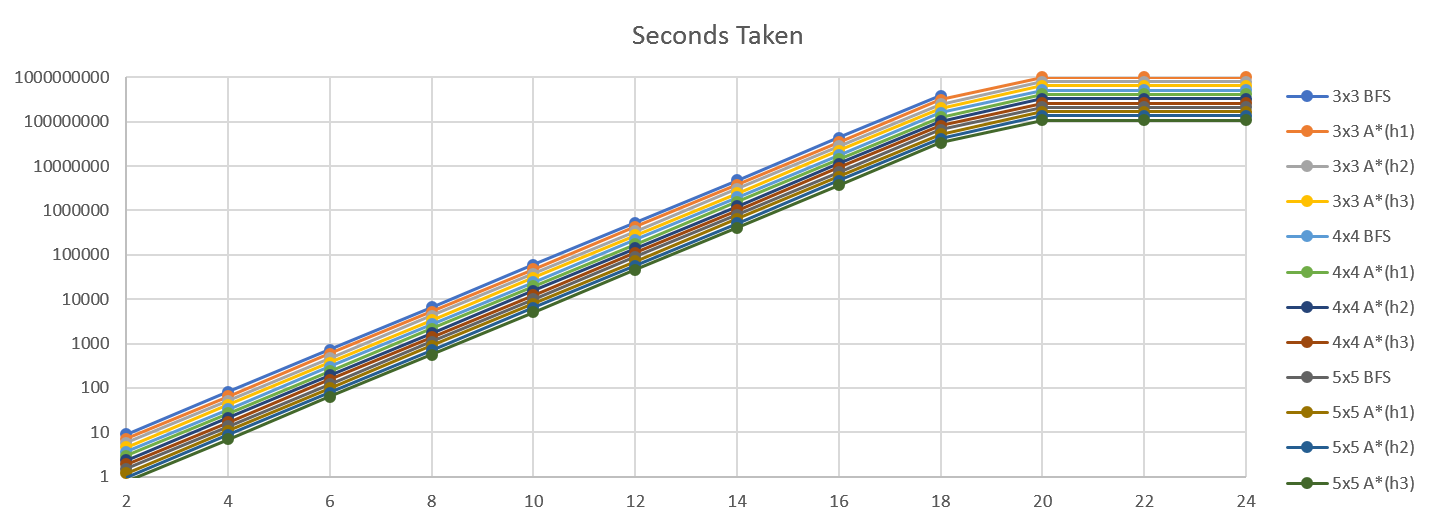
\includegraphics[width=\textwidth]{results_time.png}
	%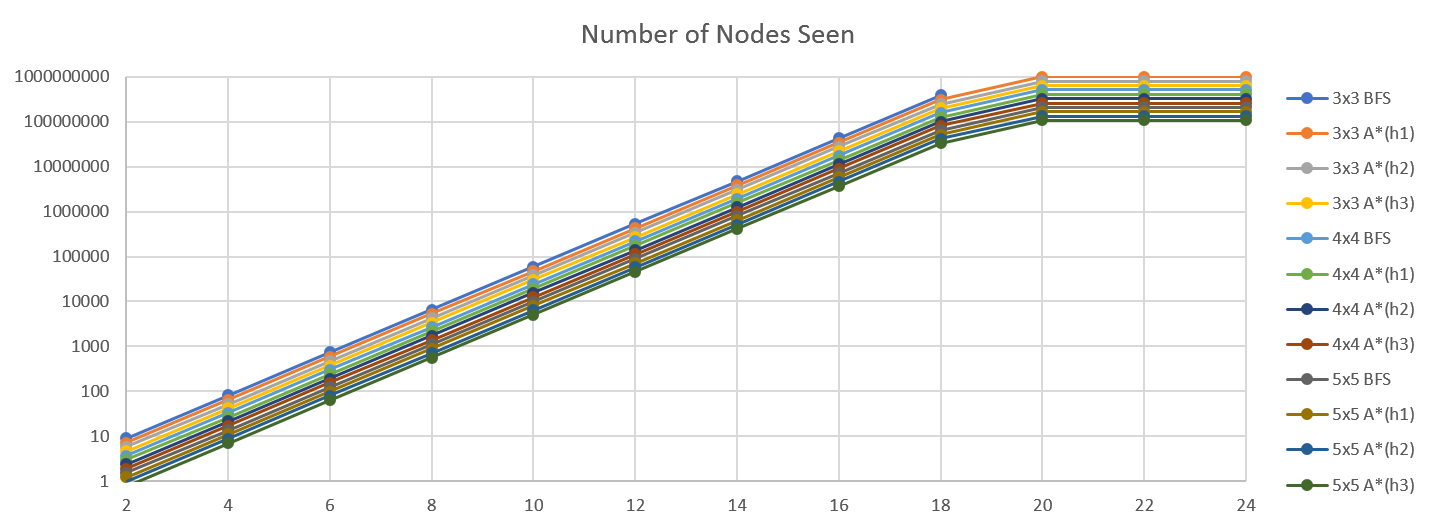
\includegraphics[width=\textwidth]{results_space.png}
	\caption{Plot of the performance results of the proposed algorithms.} \label{fig:results}
\end{figure}



\section{Results and Discussion}
The average time and space complexities for all algorithms are $O(1.667^d)$ for 3x3, $O(2^d)$ for 4x4, and $O(2.2^d)$ for 5x5. (See see \ref{subsec:branchingfactors} for the average branching factor.) The empirical results in Figure \ref{fig:results} supports this analysis.

Figure \ref{fig:results} also shows that the algorithms in order of most to least time-efficient is A* with $h_3$, A* with $h_1$, A* with $h_2$, then finally BFS. This agrees with our theoretical analysis regarding the dominance of one heuristic over another (where BFS may be regarded as A* with a heuristic that returns 0 everywhere).

% Announcement: ``Your report should at least be 2 pages long, and no longer than 4 pages''



% If there was a more lax report length requirement, it could be neater to split this into a time table and #nodes table
\begin{table}[p]
\centering
\caption{Performance results of the proposed algorithms.}
\label{tab:aresults}
\begin{tabular}{|c|
		>{\centering}p{0.105\textwidth}|>{\centering}p{0.095\textwidth}|
		>{\centering}p{0.105\textwidth}|>{\centering}p{0.095\textwidth}|
		>{\centering}p{0.105\textwidth}|>{\centering}p{0.095\textwidth}|
		>{\centering}p{0.105\textwidth}|>{\centering\arraybackslash}p{0.095\textwidth}|} % compile error without \arraybackslash for some reason
\hline
      3x3
      & \multicolumn{2}{c|}{BFS} & \multicolumn{2}{c|}{A* with $h_1$} & \multicolumn{2}{c|}{A* with $h_2$} & \multicolumn{2}{c|}{A* with $h_3$} \\
\hline
Depth $d$ & Time taken (s) & \#Nodes seen & Time taken (s) & \#Nodes seen & Time taken (s) & \#Nodes seen & Time taken (s) & \#Nodes seen \\
\hline
 2  & 1 & 1 & 1 & 1 & 1 & 1 & 1 & 1 \\
 4  & 1 & 1 & 1 & 1 & 1 & 1 & 1 & 1 \\
 6  & 1 & 1 & 1 & 1 & 1 & 1 & 1 & 1 \\
 8  & 1 & 1 & 1 & 1 & 1 & 1 & 1 & 1 \\
10  & 1 & 1 & 1 & 1 & 1 & 1 & 1 & 1 \\
12  & 1 & 1 & 1 & 1 & 1 & 1 & 1 & 1 \\
14  & 1 & 1 & 1 & 1 & 1 & 1 & 1 & 1 \\
16  & 1 & 1 & 1 & 1 & 1 & 1 & 1 & 1 \\
18  & 1 & 1 & 1 & 1 & 1 & 1 & 1 & 1 \\
20  & 1 & 1 & 1 & 1 & 1 & 1 & 1 & 1 \\
22  & 1 & 1 & 1 & 1 & 1 & 1 & 1 & 1 \\
24  & 1 & 1 & 1 & 1 & 1 & 1 & 1 & 1 \\
\hline
\end{tabular}
\begin{tabular}{|c|
		>{\centering}p{0.105\textwidth}|>{\centering}p{0.095\textwidth}|
		>{\centering}p{0.105\textwidth}|>{\centering}p{0.095\textwidth}|
		>{\centering}p{0.105\textwidth}|>{\centering}p{0.095\textwidth}|
		>{\centering}p{0.105\textwidth}|>{\centering\arraybackslash}p{0.095\textwidth}|}
\hline
      4x4
      & \multicolumn{2}{c|}{BFS} & \multicolumn{2}{c|}{A* with $h_1$} & \multicolumn{2}{c|}{A* with $h_2$} & \multicolumn{2}{c|}{A* with $h_3$} \\
\hline
Depth $d$ & Time taken (s) & \#Nodes seen & Time taken (s) & \#Nodes seen & Time taken (s) & \#Nodes seen & Time taken (s) & \#Nodes seen \\
\hline
 2  & 1 & 1 & 1 & 1 & 1 & 1 & 1 & 1 \\
 4  & 1 & 1 & 1 & 1 & 1 & 1 & 1 & 1 \\
 6  & 1 & 1 & 1 & 1 & 1 & 1 & 1 & 1 \\
 8  & 1 & 1 & 1 & 1 & 1 & 1 & 1 & 1 \\
10  & 1 & 1 & 1 & 1 & 1 & 1 & 1 & 1 \\
12  & 1 & 1 & 1 & 1 & 1 & 1 & 1 & 1 \\
14  & 1 & 1 & 1 & 1 & 1 & 1 & 1 & 1 \\
16  & 1 & 1 & 1 & 1 & 1 & 1 & 1 & 1 \\
18  & 1 & 1 & 1 & 1 & 1 & 1 & 1 & 1 \\
20  & 1 & 1 & 1 & 1 & 1 & 1 & 1 & 1 \\
22  & 1 & 1 & 1 & 1 & 1 & 1 & 1 & 1 \\
24  & 1 & 1 & 1 & 1 & 1 & 1 & 1 & 1 \\
\hline
\end{tabular}
\begin{tabular}{|c|
		>{\centering}p{0.105\textwidth}|>{\centering}p{0.095\textwidth}|
		>{\centering}p{0.105\textwidth}|>{\centering}p{0.095\textwidth}|
		>{\centering}p{0.105\textwidth}|>{\centering}p{0.095\textwidth}|
		>{\centering}p{0.105\textwidth}|>{\centering\arraybackslash}p{0.095\textwidth}|}
\hline
      5x5
      & \multicolumn{2}{c|}{BFS} & \multicolumn{2}{c|}{A* with $h_1$} & \multicolumn{2}{c|}{A* with $h_2$} & \multicolumn{2}{c|}{A* with $h_3$} \\
\hline
Depth $d$ & Time taken (s) & \#Nodes seen & Time taken (s) & \#Nodes seen & Time taken (s) & \#Nodes seen & Time taken (s) & \#Nodes seen \\
\hline
 2  & 1 & 1 & 1 & 1 & 1 & 1 & 1 & 1 \\
 4  & 1 & 1 & 1 & 1 & 1 & 1 & 1 & 1 \\
 6  & 1 & 1 & 1 & 1 & 1 & 1 & 1 & 1 \\
 8  & 1 & 1 & 1 & 1 & 1 & 1 & 1 & 1 \\
10  & 1 & 1 & 1 & 1 & 1 & 1 & 1 & 1 \\
12  & 1 & 1 & 1 & 1 & 1 & 1 & 1 & 1 \\
14  & 1 & 1 & 1 & 1 & 1 & 1 & 1 & 1 \\
16  & 1 & 1 & 1 & 1 & 1 & 1 & 1 & 1 \\
18  & 1 & 1 & 1 & 1 & 1 & 1 & 1 & 1 \\
20  & 1 & 1 & 1 & 1 & 1 & 1 & 1 & 1 \\
22  & 1 & 1 & 1 & 1 & 1 & 1 & 1 & 1 \\
24  & 1 & 1 & 1 & 1 & 1 & 1 & 1 & 1 \\
\hline
\end{tabular}
\end{table}



\pagebreak
\appendix
\section{Appendix: Proofs}
\label{app:proofs}
%\noindent Displayed equations are centered and set on a separate line.
%\begin{equation}
%x + y = z
%\end{equation}

% the environments 'definition', 'lemma', 'proposition', 'corollary',
% 'remark', and 'example' are defined in the LLNCS documentclass as well.

\subsection{Maximum and Average Branching Factors}
When determining the branching factor, backtracking actions that lead right back to the previous state are discounted, as that state has already been explored. This reduces the possible number of actions in all cases by 1, except for the initial state. However, the initial state incurs only a constant factor with regards to complexity analysis of the search tree, thus it can be safely ignored.

\label{subsec:branchingfactors}
\paragraph{Maximum branching factor.} Given any valid state, there are up to $|A|=4$ possible actions. After discounting backtracking actions, the maximum branching factor $b = |A|-1 = 3$. $\qed$

Note: In the case $n=2$, each cell is a corner cell and thus has only 2 actions, and 1 of them backtracks and thus is discounted. Thus $b = 1$ in this case. The complexities evaluated as $O(b^d)$ become wrong in this case as $O(1^d) = O(1)$, and they should be $O(d)$ instead.

\paragraph{Average branching factor.} Given $n$, there are $4$ corner cells of 2 branches each, $4(n-2)$ side cells of 3 branches each, and $(n-2)^2$ center cells of 4 branches each. Discount the backtracking action from each case. Assuming all states are equally likely to occur, the average branching factor $b_\text{avg}$ is thus $\frac{1\cdot 4 + 2\cdot 4(n-2) + 3\cdot (n-2)^2}{n^2} = \frac{4 + 8n - 16 + 3n^2 - 12n + 12}{n^2} = \frac{3n^2 - 4n}{n^2} = 3 - \frac{4}{n}$. $\qed$

\begin{table}[h]
\centering
\caption{Average branching factor for some values of $n$.}
\label{tab:results}
\begin{tabular}{|c||c|c|c|c|c|c|c|} \hline
$n$            & 2 & 3   & 4 & 5   & 6   &  7   & 8 \\ \hline
$b_\text{avg}$ & 1 & 5/3 & 2 & 2.2 & 7/3 & 17/7 & 2.5 \\ \hline
\end{tabular}
\end{table}

\subsection{Solvability of an Initial State \cite{Solvability}}
\label{subsec:solvability}
\begin{definition}\label{def:inversion}
For any given state $v$, write out its entries in a sequence $S(v)$, ignoring the empty cell. i.e. $S(v)_i = v_{(\lceil i/n\rceil, ((i-1) \mod n) +1)}$ for $i \in \bbbz_{[1,n^2]}$, then remove the empty cell from $S(v)$ (so it is now indexed from $1$ to $k$). An \textbf{inversion} is a pair of indices $(i,j)$ such that $i < j$, but $S(v)_i > S(v)_j$.
\end{definition}
Every state $v$ has a well-defined number of distinct inversions, denote it $I(v)$. $I(v)$ can be calculated by tallying how many distinct pairs in $v$ are inversions, which takes $O(k^2)$ time as there are $^kC_2 = \frac{k(k+1)}{2}$ pairs to check.

Given a state $v$, let $e_r(v) = n - x_e(v)$ be the row of the empty cell as counted from the bottom, and starting at 0.

\begin{theorem}\label{thm:solvability}
An initial state $s$ is solvable if and only if one of the following (mutually exclusive) cases is true:
\begin{enumerate}
\item $n$ is odd and $I(s)$ is even.
\item $n$ is even, and $I(s)$ has the same parity as $e_r(s)$.
\end{enumerate}
\end{theorem}
\paragraph{$(\implies)$}
A solvable state is one that can reach the goal state $g$ in a finite number of actions. Since each action is reversible by an opposite action, this can be restated as: A state is solvable if and only if it is reachable from $g$ in a finite number of actions.

Now given a solvable initial state $s$, consider a sequence of actions taken to move from $g$ to $s$, and how $I(v)$ changes across it. For each action, consider its start state $v$ and result state $v'$.

If an action moves horizontally, $S(v) = S(v')$, thus $I(v') = I(v)$.

If an action moves vertically, then $n-1$ swaps between adjacent elements occur from $S(v)$ to $S(v')$, and each swap either introduces or resolves an inversion, which flips the parity of $I(v')$.

If $n$ is odd, then the number of swaps $n-1$ is even and thus the parity of $I(v')$ is always the same as $I(v)$. Thus, the parity of $I(v)$ stays the same over the entire path from $g$ to $s$. Therefore, $I(s)$ has the same parity as $I(g)$. And $I(g) = 0$ is even.

If $n$ is even, then $n-1$ is odd and thus the parity of $I(v')$ is always different from $I(v)$ (when the action is vertical).

If $e_r(s)$ is even (resp. odd), then the number of vertical actions taken to get to $g$ is even (resp. odd) as well. Thus, the parity of $I(v)$ flips an even (resp. odd) number of times over the entire path from $g$ to $s$. Therefore, $I(s)$ has the same (resp. different) parity as $I(g) = 0$, which is even.
$\qed$

\paragraph{$(\impliedby)$}
This is essentially a tedious proof by construction, and the proof is deferred. The general strategy is to move 1 to the right place and never move it again, then do the same with 2, then 3, and so on, up until the puzzle is solved.
$\qed$



%Multiple citations: \cite{ref_article1,ref_book1,ref_proc1,ref_url1}

% ---- Bibliography ----
% BibTeX users should specify bibliography style 'splncs04'.
% References will then be sorted and formatted in the correct style.
\bibliographystyle{splncs04}
\bibliography{reportbib}

\end{document}
